\documentclass{iitthesis}


% Document Options:
%
% Note if you want to save paper when printing drafts,
% replace the above line by
%
%   \documentclass[draft]{iitthesis}
%
% See Help file for more about options.

\usepackage{graphicx}    % This package is used for Figures
\usepackage{rotating}

\begin{document}

%%% Declarations for Title Page %%%
\title{Acceptance of Code Contributors on GitHub}
\author{Matthew Heston}
\degree{Master of Science}
\dept{Information Architecture}
\date{May 2014}
% \copyrightnoticetrue      % crate copyright page or not
%\coadvisortrue           % add co-advisor. activate it by removing % symbol to add co-advisor
\maketitle                % create title and copyright pages


\prelimpages         % Settings of preliminary pages are done with \prelimpages command


%%%  Acknowledgement %%%
\begin{acknowledgement}     % acknowledgement environment, this is optional
\par  This dissertation could not have been written without Dr. X
who not only served as my supervisor but also encouraged and
challenged me throughout my academic program. He and the other
faculty members, Dr. Y and Dr. Z, guided me through the
dissertation process, never accepting less than my best efforts. I
thank them all.\\ \\ (Don't copy this sample text. Write your own
acknowledgement.)
% or \input{acknowledgement.tex} % you need a separate acknowledgement.tex file to include it.
\end{acknowledgement}


% Table of Contents
\tableofcontents
\clearpage

% List of Tables
\listoftables

\clearpage

%List of Figures
\listoffigures

\clearpage

%List of Symbols(optional)

% \listofsymbols
%  \SymbolDefinition{$\beta$}{probability of non-detecting bad data}
%  \SymbolDefinition{$\delta$}{Transition Coefficient Constant for the Design of Linear-Phase FIR Filters}
%  \SymbolDefinition{$\zeta$}{Reflection Coefficient Parameter}


%  \clearpage



%%% Abstract %%%
\begin{abstract}           % abstract environment, this is optional
\par Your Abstract goes here!
% or \input{abstract.tex}  %you need a separate abstract.tex file to include it.
\end{abstract}


\textpages     % Settings of text-pages are done with \textpages command

% Chapters are created with \Chapter{title} command
\Chapter{INTRODUCTION}

GitHub is a social website that open source software developers use to host
their software projects and to browse other developers' projects. It includes
many features that are present on social networking sites, such as the ability
to follow other users and leave comments on projects. GitHub provides a wealth
of data for studying computer supported cooperative work, as it is a
centralized location where many different tasks take place. For example, users
can create bug reports, submit fixes, and engage in discussions about new
features all on one website.  In this study, we use statistical and machine
learning methods on data from GitHub repositories to explore how different
factors may affect the acceptance of code changes from first time contributors.

The rest of this paper is organized as follows. The rest of this chapter
provides a literature review on the subject, establishing the importance of
studying open source software development, situating it within a context of
virtual work and computer mediated communication, and reviewing a theoretical
basis we use to inform our empirical methods. Chapter~\ref{chap:methods}
describes our data collection and data analysis methods. The results of our
experiments are discussed in Chapter~\ref{chap:results}. We conclude in
Chapter~\ref{chap:conclusion} and discuss opportunities for future work.


\Section{Related Work} \label{sec:relatedwork}

\Subsection{FLOSS Research}
Research in the development of free/libre open source software (FLOSS) has
grown tremendously in the last several years. Crowston et
al.~\cite{crowston_free/libre_2008} note the importance of understanding FLOSS
development as it becomes a major social movement with many volunteers
contributing to projects, and many FLOSS projects becoming integral parts of the
infrastructure of modern societ as it becomes a major social movement with many
volunteers contributing to projects, and many FLOSS projects becoming
integral parts of the infrastructure of modern society. Other studies have
emphasized the role that FLOSS research can play in improving current existing
research of software engineering, particularly as the importance of
understanding large scale software systems in science and insustry
increases ~\cite{scacchi_free/open_2007}.

Existing research approaches FLOSS from many different angles, including
motivation of open source
developers~\cite{fang_understanding_2009},
~\cite{lakhani_why_2003},~\cite{shah_motivation_2006}; governance of open souce
projects~\cite{hippel_open_2003},~\cite{omahony_guarding_2003},~\cite{omahoney_governance_2007};
and knowledge sharing within FLOSS
communities~\cite{endres_tacit_2007},~\cite{hemetsberger_collective_2009},~\cite{sowe_understanding_2008}.
Our study focuses on the behavior of first time contributors to FLOSS projects
and community response to their contributions. We build on previous studies that
describe the social processes of community
joining~\cite{ducheneaut_socialization_2005},~\cite{huang_mining_2005}, ~\cite{von_krogh_community_2003}. Given the
distributed nature of FLOSS development, our findings contribute to current
descriptions of virtual work and distributed teams.
%TODO new members

Previous studies have used version control histories to verify learning
processes of new members in FLOSS projects~\cite{huang_mining_2005}. GitHub,
however, has not been extensively studied as it is a relatively new social
platform. Dabbish et al.~\cite{dabbish_social_2012} study how GitHub as a social
application provides transparency and how that transparency affects
collaboration and learning. McDonald and
Goggins~\cite{mcdonald_performance_2013} study how different communities on
GitHub measure success. Choi et al.~\cite{choi_herding_2013} study a sample of
GitHub based projects to contribute to theories of developer coordination. In
all these cases, the social features of GitHub, e.g. the ability to follow other
users and view information about them, provide new ways to study social behavior
in FLOSS projects. Our study investigates members' participation in group
discussions on the site. While previous studies have tried to combine data from
mailing lists and version control~\cite{ducheneaut_socialization_2005}, GitHub
provides a centralized location to study communities in which discussion and
code contribution all occur in one place. At least with regards to user support,
recent research suggests that developers may be moving away from mailing lists
to social Q\&A sites to respond to user requests for
help~\cite{vasilescu_how_2014}. By focusing on GitHub data, we contribute to
understanding developer behavior on this new social platform.


\Subsection{Communities of Practice} \label{sec:communities}
Our study focuses on the behavior of new code contributors and community
response to their contributions. We use the theoretical framework of
\textit{legitimate peripheral participation} (LPP) ~\cite{lave_situated_1991} in
our exploration community joining. LPP describes a process of learning in
communities of practice in which newcomers join a community by participating in
peripheral tasks and forming relationships to move towards the center of the
community. Several studies of FLOSS development have used the LPP framework.
Huang and Liu~\cite{huang_mining_2005} mine version control history to construct
developer networks and identify core and peripheral community members.
Ducheneaut~\cite{ducheneaut_socialization_2005} finds a pattern that resembles
LPP in his study of contributors to the Python project. Ye and
Kishida~\cite{ye_toward_2003} use LPP to ground their theory of motivation in
open source communities. This concept has been explored in other studies of
computer mediated communication.  In their study on members of Wikipedia,
~\cite{bryant_becoming_2005} note that members initially become involved through
peripheral activities. These are simple and low risk activities members can take
part in to learn more about the community before trying to become major
contributors. Similarly, ~\cite{von_krogh_community_2003} from observing open
source communities generate the construct of a \textit{joining script}, where
each project has a set of tasks for new developers to go through before being
accepted into the community.

Our study seeks to which factors contribute to the acceptance of code
contributions of first time contributors. We use LPP as a theoretical framework
to ground our experiments.

\Chapter{METHODS} \label{chap:methods}

\Section{Terminology} \label{sec:terms}

A software project on the website is referred to as a \textit{repository}. Any
user on GitHub can \textit{star} a repository. Users star repositories to be
able to easily navigate to it and to receieve updates on activity from the
repository. If a developer wants to contribute to another one of developer's
repositories, he can \textit{fork} the repository, which creates a copy of the
project for him to work on. As the developer makes changes to this code, he
\textit{commits} his changes. A \textit{commit} is a snapshot of the code at a
certain point in time. When the developer is finished, he can submit a
\textit{pull request} to the owner of the project. All pull requests for a
project are viewable on GitHub, and any user of the site can comment on them. A
pull request can have a status of open or closed. A status of open indicates
that that owner of the repository has not made a decision about whether or not
to include the changes. If the owner of a repository wants to incorporate the
changes the developer made, he can \textit{merge} them into the repository. A
pull request can be closed without being merged, which means that the changes
the developer made were not accepted.

\Section{Data Collection} \label{sec:datacollection}

Data was collected using the GitHub API.\footnote{http://developer.github.com/}
We used a collection of node.js scripts to collect data from the API to store in
a MySQL database.\footnote{These scripts are available at
http://www.github.com/matthewheston/gh-collector.} In selecting which
repositories to use for our analysis, we started with the top 100 most starred
repositories on GitHub. We started with this list with the assumption that they
were popular repositories that would be maintained by an active community. From
these 100, we manually filtered out certain projects that we expected would
follow different development patterns than a typical programming project, for
example, collections of configuration files for text editors and shells,
collections of icons, etc. We also excluded repositories that were used
primarily for demonstration or documentation purposes, such as sample web
applications to demonstrate use of a certain web framework. After filtering our
intial list of 100, 45 repositories remained in our data set for analysis. We
only consider pull requests with a status of closed. This resulted in
approximately 44,400 pull requests. We further filtered this data by select only
the first pull request a user submitted to a repository, leaving 13,383 pull
requests. The distribution of these pull requests across repositories ranges
from 10 to 1,489, with a median of 210. To find merged pull requests, we first
filter all pull requests that are marked as merged by the GitHub API, meaning
that the project maintainers used GitHub's merge feature to accept the pull
request. In some repositories, project maintainers use a different workflow when
accepting pull requests, wherein the code changes are accepted, but it is not
reflected as merged on GitHub. In most of these cases, there is a standard way
of reflecting this in the commit comments, so we use some naive heuristics for
identifying these requests by searching commit comments for certain text
patterns. For example, in many projects, the project maintainer will manually
add the commits from the pull request, and create a new commit with a commit
message that follows the pattern "Closes {number}" where {number} is the pull
request ID on GitHub. Finding merged pull requests using both the status from
the GitHub API as well as these text patterns results in finding 5,239, or
39.1\% of first pull requests being merged.

\Section{Data Analysis} \label{sec:data_analysis}

We divide our analyis into two dimensions: community engagement of developer and
communtiy response. Our research questions our presented in
Table~\ref{research_questions}, along with a summary of the variables and
methods we used.

\begin{sidewaystable}[ht] \centering \label{tbl:research_questions}
\caption{Summary of research questions and methods.}
\begin{tabular}{ p{3in} p{3in} p{2in} }
\hline\hline
Research Question
& Data                                  & Measure
\\
How does a user engage before submitting their first pull request?
& Comments on other pull requests.      & We plot the total number
of pull requests a user has commented on the x-axis of
Figure~\ref{fig:aprr_up}.
\\
Does community response affect whether or not a pull request is
merged? & Number of comments on pull request.   & We plot the
total number of comments for submitted pull requests on the
y-axis of Figure~\ref{fig:aprr_up}.
\\
~
& Language in comments on pull request. & We train both a
logistic regression and naive bayes classifier after
converting comments on submitted pull requests to feature
vectors. Results are shown in
Table~\ref{tbl:classifiers} \\
\hline
\end{tabular}
\end{sidewaystable}

\Subsection{Community Engagement of Developer}
To explore the process of legitimate peripheral participation discussed in
Section~\ref{sec:communities}, we count the total number of pull requests a
developer commented on before submitting his own pull request. We consider
commenting on other pull requests the primary peripheral activity a user can
participate in. This variable is shown in the x-axis of
Figure~\ref{fig:aprr_up}.

\begin{figure}[p] \centering \label{fig:aprr_up}
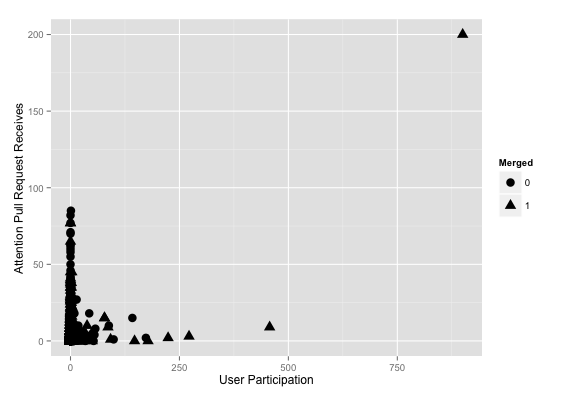
\includegraphics[scale=0.6]{figures/aprr_up_ggplot.png} \caption{User
participation and attention a pull request recieves for all first pull
requests.} \end{figure}

\Subsection{Community Response}
In addition to measuring the activity of a developer in the community before
submitting a pull request, we are also interested in measuring the community
response to a given pull request and how that response relates to whether or not
a pull request is accepted. We measure this in two ways.

First, we simply count the number of comments on a given pull request. This is
used as a basic metric of how much attention a pull request receives. This
variable is shown on the y-axis of Figure~\ref{fig:aprr_up}.

Our next analysis of community response focuses on the language of the comments
on a pull request. To test whether or not the content of these comments is
predictive of whether or not a pull request is merged, we collect the comments
for each of our first pull requests. We ignore comments made by the user who
submitted the pull request, since we are interested in what other users had to
say about it. We also ignore the last comment associated with a pull request,
since these often will explicitly say whether or not the maintainer is merging
the pull request or not.  We are interested in whether the type of language used
in the discussion of a pull request is predictive of whether or not it is
accepted. We ignore pull requests that only have one comment associated with it.
This leaves 5,674 pull requests. 3,811, approximately 67\% were not accepted. We
treat the remaining comments associated with the pull request as one document,
and convert them into feature vectors representing the count of each unigram and
bigram in the documents, and train both a logistic regression and naive bayes
classifier using this feature set. The results of testing these classifiers is
shown in Table~\ref{tbl:classifiers}. The results shown are the result of
running 10-fold cross validation.

\begin{table}[ht] \centering \label{tbl:classifiers}
  \caption{Classifier results}
  \begin{tabular}{lll}
  \hline\hline
  ~         & Logistic Regression & Naive Bayes \\
  Accuracy  & 69.6\%              & 70.6\%      \\
  Precision & 56.0\%              & 60.3\%      \\
  Recall    & 36.1\%              & 30.7\%      \\
  \hline
  \end{tabular}
\end{table}

\Chapter{RESULTS} \label{chap:results}

\Section{Community Engagement of Developer}

We see that user participation for the majority of all first pull requests, both
merged and not merged, is 0. This indicates that in general, most users are not
attempting to engage in the peripheral activity of commenting on other pull
requests before submitting their own. The GitHub interface makes it relatively
easy for a user to fork a repository, make changes, and submit the changes for
consideration. Previous studies on GitHub have shown that the number of
contributions did increase for some projects that moved from other hosting
options to GitHub~\cite{mcdonald_performance_2013}. It is possible this
interface lowers the barrier of entry for a developer who wants to contribute to
a project, and allows them to bypass participating in the joining script
described by von Krogh et al. ~\cite{von_krogh_community_2003}.

We also examine these variables for first pull requests by users who later
submit another pull request. We want to see whether or not this no engagement
pattern continues to hold for users who will become active contributors. Our
intuition here is that some users might encounter a bug they fix or desire a
feature that they implement, and then submit these changes back to repository.
They may not comment on other pull requests as they are not interested in
becoming long term members of the community, but rather are just interested in
submitting a one time patch. Users who do plan on becoming active members,
however, may participate in peripheral activities more.
Figure~\ref{fig:aprr_up_repeaters} shows a visualization of the same first pull
requests, but only for users who submit at least one other pull request at a
later point in our data set, and Figure~\ref{fig:aprr_up_repeaters_10} shows the
data for users who submit at least 5 more times. Looking at users who submit at
least one other time cuts our number of observations from 13,383 to 5,207,
indicating that approximately 61\% of these pull requests come from users who
will not contribute any others. Looking at users who will submit at least 10
more times gives us a total of 1,155 observations.

It is clear that in all these cases, regardless of whether or not they will be
continuing to submit other pull requests later, at the time of submitting their
first pull request, users are generally not participating in the community. The
previous graphs only consider the number of pull requests a user commented on
before submitting their first pull request, so we do not capture how users who
submit multiple pull request over time comment on other pull requests over time.
In Figure~\ref{fig:commented_pullrequests_totals} we plot the total number of
others' pull requests that a user commented on by how many pull requests they
submitted themselves, considering only users who have submitted at least two
pull requests. There is not a strong correlation between these variables
(Spearman's $\rho$  = 0.44), indicating that users do not necessarily
participate in more commenting as they continue to submit more pull requests.

It's worth noting the one extreme outlier present in
Figures~\ref{fig:aprr_up}, ~\ref{fig:aprr_up_repeaters}, and
~\ref{fig:aprr_up_repeaters_10}. This is an interesting case of a project
maintainer, who has commit access and wouldn't typically need to submit a pull
request to submit changes, creating a pull request for commits related to a
major upgrade in the project. By creating a pull request, he was able to
document all the changes associated with this change and allow community members
to ask questions or comment on the changes. He has a high number of previous
comments since he is in charge of accepting pull requests. Due to the nature of
this pull request, there is a high number of comments on this pull requests on
it, since many other developers are asking questions or voicing their opinions.
This is a useful example that demonstrates the different ways pull requests may
be used in different projects, and how the way they are used may change
depending on the type of user submitting them.

\begin{figure}[p] \centering \label{fig:aprr_up_repeaters}
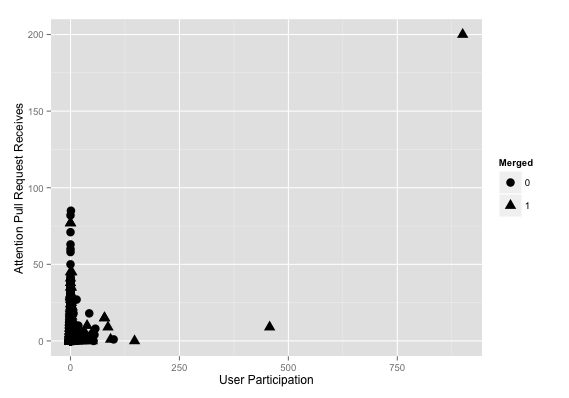
\includegraphics[scale=0.6]{figures/aprr_up_repeaters_ggplot.png} \caption{User
participation and attention a pull request recieves variables for users who
submit at least one other pull request in our data set.} \end{figure}

\begin{figure}[p] \centering \label{fig:aprr_up_repeaters_10}
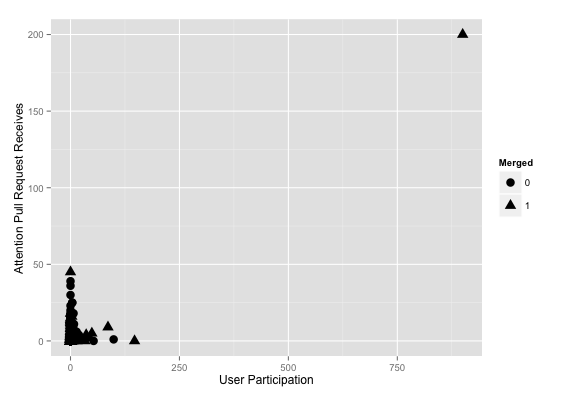
\includegraphics[scale=0.6]{figures/aprr_up_repeaters_10_ggplot.png}
\caption{User participation and attention a pull request recieves variables for
users who submit at least 10 other pull requests in our data set.} \end{figure}

\begin{figure}[p] \centering \label{fig:commented_pullrequests_totals}
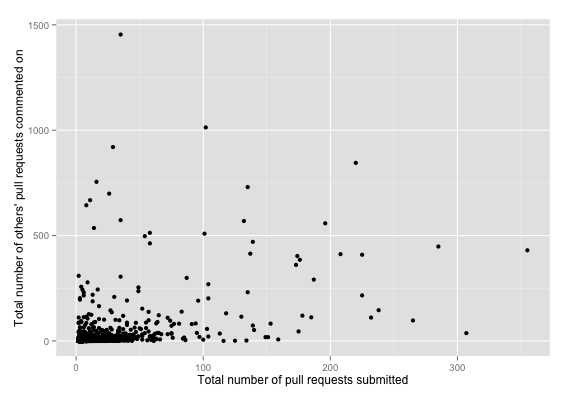
\includegraphics[scale=0.6]{figures/commented_pullrequests_totals_ggplot.png}
\caption{Total number of pull requests commented on and total number of pull
requests submitted for each user.} \end{figure}

\Section{Community Response}
In Figure~\ref{fig:aprr_up}, we see more variance in the number of comments on
first pull requests than we did with the number of pull requests users commented
on before submitting. However, there is clearly no linear separation of merged
and not merged pull requests using this variable, so it seems just viewing the
amount of activity a pull request receives is not enough to explain whether or
not it gets merged.

Training classifiers using the comment text may help address this problem, as
this can capture the valence of the comments, rather than just the raw number.
However, the low recall rates we see in Table~\ref{tbl:classifiers} indicate
that the text data is not sufficient to distinguish positive cases. Of course,
our sample size of 5,674 is relatively small, but it is interesting to note that
only 42\% of the first pull requests in our data set have more than 1 comment
associated with them. Our research question that drove these experiments was how
community response affects whether or not a pull request is accepted. However,
we see that the majority of pull requests don't attract any community attention.

\Chapter{Conclusion} \label{chap:conclusion}

In this study, we analyzed community engagement and community response of first
time code contributors on GitHub. We found that most developers do not engage by
participating in discussions on GitHub before submitting code changes. We also
find that most submitted pull requests do not attract much community response,
and our attempts at measuring communtiy response do not provide good predictors
for whether or not a pull request is accepted. Our findings have implications
for researchers, open source contributors, and open source project maintainers.

We found that most users do not engage with the community in the way we expected
from previous FLOSS and LPP literature. Some reasons for this are discussed
below in Section~\ref{sec:future_work}. Since GitHub is a new platform that
encourages new types of social interactions, it can be used as a new source of
data to study open source communities. Our study focused on a relatively small
number of repositories pulled from the most starred repositories on GitHub.
Further work should be done on a larger sample of different types of
repositories. It's possible that new types of social websites like GitHub will
require new theoretical ways of thinking about distributed work and virtual
teams.

The majority of first pull requests in our data set were not accepted, but
community engagement is not a good predictor or whether or not they are
accepted, and most developers do not engage before submitting a pull request,
even if they end up becoming active code contributors. The implication for
developers who want to become involved in an open source project on GitHub is
that they do not necessarily need to participate in peripheral activities before
submitting pull requests. Although our study did not identify which factors do
contribute to acceptance of pull request, it's possible that developers should
focus more on things like finding relevant issues to fix or features to work on
rather than on social interactions.

Many open source projects fail due to insufficient volunteer
participation~\cite{crowston_defining_2003},~\cite{krishnamurthy_cave_2002}. It
is therefore important for project maintainers to continue to attract volunteer
developers to keep a project alive. We found that 61\% of first pull requests
in our data set come from users who will not submit any other pull requests.
Project owners should consider ways to convert these one time contributers to
regular active contributors.

\Section{Future Work} \label{sec:future_work}

Our major finding in this study is that, despite previous FLOSS research which
did indicate social patterns that follow legitimate peripheral participation
framework~\cite{ducheneaut_socialization_2005},~\cite{huang_mining_2005},~\cite{ye_toward_2003},
we generally do not see this pattern in our GitHub data set. Although some
developers do leave comments on other pull requests before submitting their own,
the majority of developers do not, including those that will continue to submit
code changes. There are many reasons this might be the case.

As mentioned in Section~\ref{results_engagement}, GitHub's interface makes it
fairly easy to submit changes. Users only need to click a button to create a
copy of the repository that they can make commits on, and then click another
button to submit those commits as a pull request when they are finished. This
process may lower barriers to entry for new developers. While previous studies
of FLOSS communities have focused on mailing lists and centralized version
control repositories, the distributed nature of git may be altering the social
patterns that take place in developer networks. This study may suggest we need
to alter existing social theory as new interfaces change social interactions.

However, this study only focused on data from GitHub, and our notion of
community engagement by developers was limited to activity by developers on
GitHub. While we have shown that this data is not sufficient to predict whether
or not a pull request is merged, further studies should create joint data sets
merging GitHub data with data from other sources, such as mailing lists, forums,
or chat rooms to test whether or not developers engage with the community using
these other platforms, and how those social interactions affect their acceptance
in the community. One difficulty in creating these types of data sets is
identify merging, the process of matching different logins from different
services to the same physical person, but a number of techniques have been
proposed to assist in this
process~\cite{bird_open_2007},~\cite{goeminne_comparison_2013},~\cite{kouters_whos_2012}.

It's also possible that looking at only social factors is not enough to
understand what contributes to acceptance on GitHub. Static analysis tools may
be used in addition to the metrics we used in this study to further explore how
the code itself affects whether or not a pull request is accepted.

In addition to studying community engagement by developers, we also examined
community response to these developers. In most cases, there was little
community response. As mentioned above, attraction of new developers and
retention of developers is important to project success. Future work should how
community response can affect developer retention in GitHub projects.

To better understand the way that the GitHub interface affects developer
behavior will require further qualitative study. While there have been surveys
of GitHub developers previously~\cite{mcdonald_performance_13}, there remains a
lot of work left to do in this area. Future quantitative studies should collect
larger samples of data and explore new ways of measuring these types of social
variables.

\clearpage


%
% APPENDIX
%

% Do the settings of appendices with \appendix command
\appendix

% Then create each appendix using
% \Appendix{title_of_appendix} command
%
% BIBLIOGRAPHY
%
% you have two options: 1) create bibliography manually,
% 2) create bibliography automatically. See BibliographyHelp.pdf file for details.


\bibliographystyle{plain}
\bibliography{Master}

\end{document}  % end of document
